\section{Introduction}
\label{sec:intro}

The self-attention mechanism~\citep{vaswani2017attention} is a cornerstone of modern large language models~(LLMs), yet its quadratic complexity in sequence length presents a fundamental bottleneck for long-context inference.
As LLMs are increasingly deployed in settings that demand extended contexts, such as long chain-of-thought reasoning, multi-step agentic workflows, and retrieval-augmented generation over web-scale sources, reducing attention cost without sacrificing model quality has become a critical research problem.

\begin{wrapfigure}{r}{0.4\linewidth}
    \centering
    \vspace{-1em}
    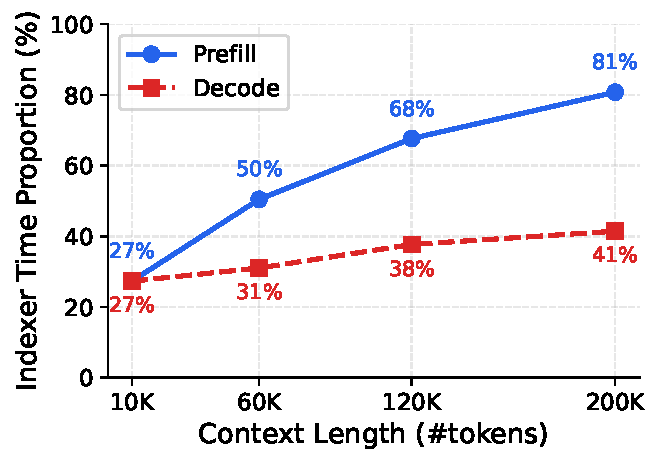
\includegraphics[width=\linewidth]{figures/indexer_time_ratio.pdf}
    \vspace{-2em}
\end{wrapfigure}
Sparse attention offers a principled solution: instead of attending to all preceding tokens, each query selects only the most relevant subset.
Among recent approaches~\citep{nsa,moba,infllm-v2,hysparse,longcat}, DeepSeek Sparse Attention~(DSA)~\citep{deepseekv32} stands out as a production-grade trainable sparse attention mechanism.
For sparse token selection, DSA introduces an additional \emph{lightning indexer} module at each layer that scores all preceding tokens and selects the top-$k$ for the subsequent core attention.
This reduces per-layer core attention from~$O(L^2)$ to~$O(Lk)$ while preserving model quality through continued pre-training.
However, the indexer itself still operates at~$O(L^2)$ at \emph{every} layer: although cheaper per-FLOP than the main attention computation, its total cost across~$N$ layers is~$O(NL^2)$, which grows quadratically with context length and becomes a non-negligible fraction of the total attention budget.
As shown in the figure above, profiling a 30B DSA model reveals that the indexer's share of total latency rises sharply with context length, particularly during the prefill stage, while the rest of the computations grow only modestly. This indicates that \textbf{reducing indexer cost is the key to accelerating long-context DSA inference}.

A key insight motivating our work is that the top-$k$ selections produced by the indexer are \emph{highly correlated across consecutive layers}---an instance of the broader cross-layer token selection stability observed in full attention models~\citep{kascade,hysparse}.
While prior methods exploit this stability by reusing indices from full attention anchor layers, they do not directly apply to sparse attention, since in DSA, full attention is only computed via the lightweight indexer.
We empirically verify this for DSA by computing the pairwise top-$k$ index overlap across all layers (Appendix~\ref{app:topk-overlap}): adjacent layers share 70-100\% of their selected tokens, and the heatmap reveals distinct layer clusters with mutually high overlap, suggesting that most indexer computations are redundant.
This leaves a simple but impactful opportunity: \emph{can we remove the majority of indexers in DSA and let most layers reuse top-$k$ indices from a small number of retained indexer layers, without degrading quality?}

We answer affirmatively with \textbf{IndexCache}, a method that eliminates up to~75\%\ of indexer computations in DSA through cross-layer index reuse.
IndexCache partitions layers into \texttt{F}~(Full) layers that retain their indexers and \texttt{S}~(Shared) layers that inherit top-$k$ indices from the nearest preceding~\texttt{F}~layer, adding only one conditional branch in inference~(Figure~\ref{fig:pseudocode-comparison}).
We propose two complementary approaches to determine and optimize this configuration:

\begin{itemize}[leftmargin=*,itemsep=4pt]
    \item \textbf{Training-free IndexCache} applies to any off-the-shelf DSA model without weight updates.
    We show that na\"{\i}ve uniform interleaving degrades quality, and propose a \emph{greedy layer selection} algorithm that uses LM loss on a small calibration set to determine the optimal pattern, namely which layers to retain indexers.
    The greedy solution retains only~$1/4$ of indexers while matching the original DSA model's downstream performance.

    \item \textbf{Training-aware IndexCache} optimizes the model \emph{parameters} for cross-layer sharing.
    We introduce a \emph{multi-layer distillation loss} that trains each retained indexer against the attention distributions of all layers it serves.
    Under this objective, even a simple uniform interleaved pattern achieves on par with the original per-layer indexer design.
\end{itemize}

Empirically, on a 30B DSA model evaluated across nine long-context and reasoning benchmarks, both training-free (with greedy pattern search) and training-aware IndexCache retain only~$1/4$ of indexers with negligible quality degradation, yielding up to \textbf{1.82$\times$}~prefill speedup and \textbf{1.48$\times$}~decode speedup at 200K context length. Preliminary results on the 744B GLM-5 further confirm scalability, achieving at least 1.3$\times$ speedup with negligible degradation in long-context performance.

\begin{figure}[t]
\centering
\begin{minipage}[t]{0.48\textwidth}
\begin{algorithm}[H]
\caption*{\textbf{(a) Standard DSA Inference}}
\begin{algorithmic}[1]
\REQUIRE Input~$\mathbf{X}$, layers~$1 \ldots N$
\FOR{$\ell = 1$ \TO $N$}
    \STATE $\mathbf{I}^{(\ell)} \leftarrow \textproc{Indexer}_\ell(\mathbf{X})$
    \STATE $\mathcal{T}^{(\ell)} \leftarrow \mathrm{Top\text{-}k}(\mathbf{I}^{(\ell)})$
    \STATE $\mathbf{X} \leftarrow \textproc{SparseAttn}_\ell(\mathbf{X},\, \mathcal{T}^{(\ell)})$
    \STATE $\mathbf{X} \leftarrow \textproc{FFN}_\ell(\mathbf{X})$ \hfill $\triangleright$~\textrm{\small + norm, residual, etc.}
\ENDFOR
\end{algorithmic}
\end{algorithm}
\end{minipage}
\hfill
\begin{minipage}[t]{0.48\textwidth}
\begin{algorithm}[H]
\caption*{\textbf{(b) IndexCache Inference}}
\begin{algorithmic}[1]
\REQUIRE Input~$\mathbf{X}$, layers~$1 \ldots N$, pattern~$\mathbf{c}$
\FOR{$\ell = 1$ \TO $N$}
    \IF{\textcolor{red}{$c_\ell = \texttt{F}$}}
        \STATE $\mathbf{I}^{(\ell)} \leftarrow \textproc{Indexer}_\ell(\mathbf{X})$
        \STATE $\mathcal{T}^{(\ell)} \leftarrow \mathrm{Top\text{-}k}(\mathbf{I}^{(\ell)})$
        \STATE \textcolor{red}{$\mathcal{T}_{\mathrm{cache}} \leftarrow \mathcal{T}^{(\ell)}$}
    \ELSE[\textcolor{red}{$c_\ell = \texttt{S}$}]
        \STATE \textcolor{red}{$\mathcal{T}^{(\ell)} \leftarrow \mathcal{T}_{\mathrm{cache}}$} \hfill \textcolor{red}{$\triangleright$~reuse}
    \ENDIF
    \STATE $\mathbf{X} \leftarrow \textproc{SparseAttn}_\ell(\mathbf{X},\, \mathcal{T}^{(\ell)})$
    \STATE $\mathbf{X} \leftarrow \textproc{FFN}_\ell(\mathbf{X})$ \hfill $\triangleright$~\textrm{\small + norm, residual, etc.}
\ENDFOR
\end{algorithmic}
\end{algorithm}
\end{minipage}
\caption{%
    Side-by-side comparison of inference loops.
    \textbf{(a)}~Standard DSA runs the lightning indexer at every layer.
    \textbf{(b)}~IndexCache adds a single \textcolor{red}{conditional branch} (red lines): \texttt{F}~layers compute and cache fresh indices; \texttt{S}~layers reuse the cached indices.
    Note that~$\mathcal{T}_{\mathrm{cache}}$ is a temporary buffer holding only the current index tensor; it is overwritten at each~\texttt{F}~layer and requires no additional GPU memory beyond what standard DSA already allocates.
}
\label{fig:pseudocode-comparison}
\end{figure}
